\documentclass{article}
	\usepackage{ctex}
    \usepackage{geometry}
        \geometry{left=2.54cm,right=2.54cm,top=2.54cm,bottom=2.54cm}
    \usepackage{graphicx}
    \usepackage{subfig}
    \usepackage{float}
    \begin{document}
	\title{\textbf{信号与系统大作业} \\ [2ex] \begin{large} \emph{小白鲸找妈妈} \end{large} }
	\author{王晗\\(2013011076)}
	\date{\today}
	\maketitle
	\section{单频信号模拟}
		\subsection{读入whalesong.wav文件,听一听声音;绘制波形,解释波形和声音的关系}
            whalesong.wav波形如下图所示:
            \begin{figure}[htb]
                \centering
                \subfloat[完整波形]
                {
                    \label{fig:origin-1}
                    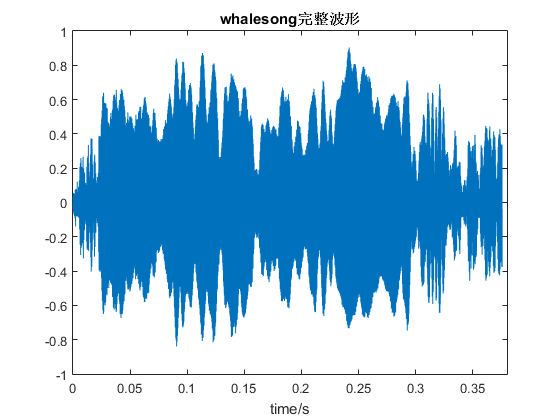
\includegraphics[width=7cm]{figure1.png}
                }
                \hspace{10pt}
                \subfloat[局部波形]
                {
                    \label{fig:origin-2}
                    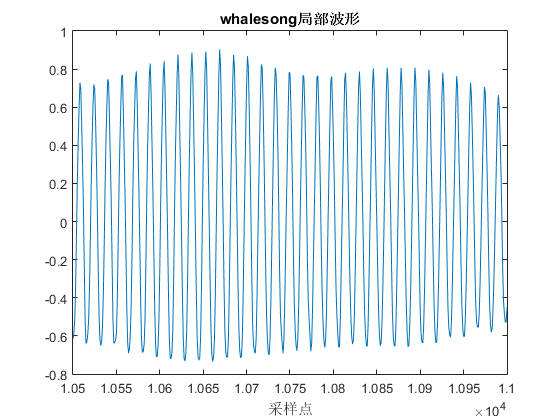
\includegraphics[width=7cm]{figure2.png}
                }
                \caption{whalesong波形}
                \label{fig:origin}
            \end{figure}

            将波形和实际的音频进行比较,可以发现波形振幅的表示声音的响度,波形的振动频率表示声音的频率。

        \subsection{如果要用一个单频信号模拟上述声音,请计算该信号的频率}
            由局部波形图计算,采样点$1.05\times10^4$ $\sim$ $1.095\times10^4$之间共有28个周期,采样频率44.1kHz,故单频信号频率:
            $$f=\frac{1}{\frac{(1.095-1.05)\times10^4}{44.1\times10^4\times28}}Hz=2744Hz$$

        \subsection{由计算得到的频率合成一个单频信号,绘制波形,听听声音,解释和白鲸的歌声有何异同}
            合成音频波形如下图所示:
            \begin{figure}[htb]
                \centering
                \subfloat[完整波形]
                {
                    \label{fig:output1-1}
                    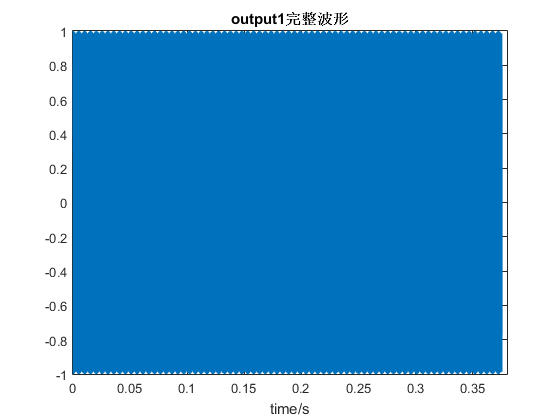
\includegraphics[width=7cm]{figure3.png}
                }
                \hspace{10pt}
                \subfloat[局部波形]
                {
                    \label{fig:synfixed-2}
                    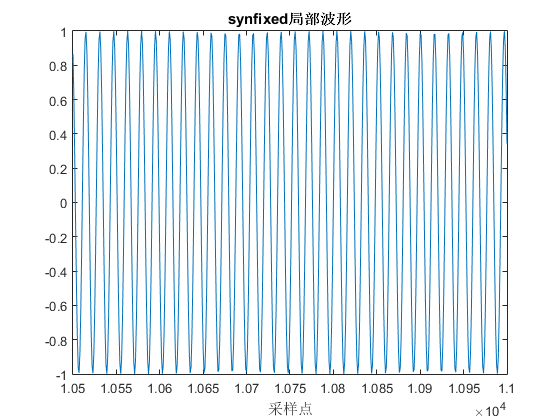
\includegraphics[width=7cm]{figure4.png}
                }
                \caption{synfixed波形}
                \label{fig:synfixed}
            \end{figure}

            单频模拟出的声音和白鲸的叫声差别较大,单频信号听起来干涩、单薄、缺乏变化,而白鲸的歌声较为饱满、通透。

        \subsection{将上述单频信号保存为synfixed.wav文件}

    \section{变频信号模拟}
        \subsection{读入whalesong.wav文件,绘制时频图,解释其含义}
            \begin{figure}[htb]
                \centering
                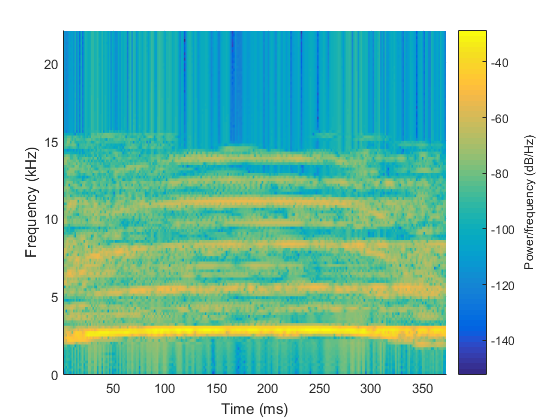
\includegraphics[width=9cm]{figure5.png}
                \label{fig:originft-1}\caption{Matlab绘制的whalesong时频图}
            \end{figure}

            \begin{figure}[!htb]
                \centering
                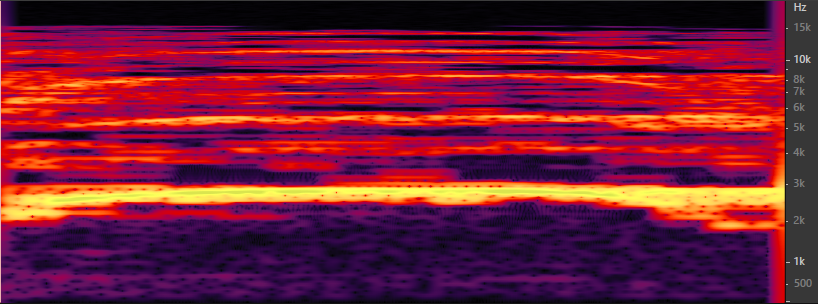
\includegraphics[width=10cm]{figure6.png}
                \label{fig:originft-2}\caption{Audition绘制的whalesong时频图}
            \end{figure}

            时频图中的颜色分布表示不同时间点上能量在频域的分布,颜色越量的区域能量越高。上图表明白鲸叫声的能量在频域主要分布在若干个频率附近。

        \subsection{如果要用一个包络和频率都随时间变化的单频信号模拟上述声音,请描述该频率变化的特征}
            1$\sim$4000采样点频率由2.25kHz线性增加至2.8kHz,幅度由0.2线性增加至1;12000$\sim$16572采样点频率由2.8kHz线性降低至1.94kHz,幅度由1线性降低至0。

        \subsection{用上题结果合成一个变频信号,绘制波形和时频图,听听声音,解释和白鲸的歌声有何异同}
            合成音频波形如下图所示:
            \begin{figure}[htb]
                \centering
                \subfloat[完整波形]
                {
                    \label{fig:synsingle-1}
                    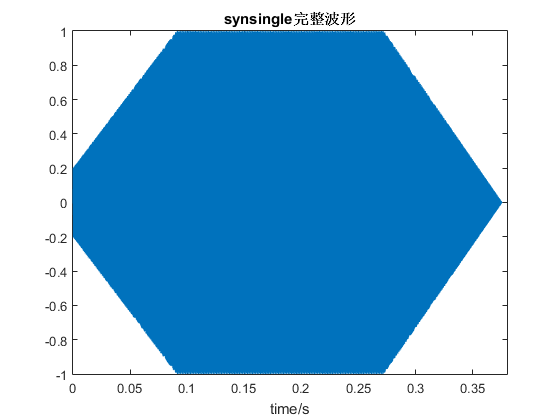
\includegraphics[width=7cm]{figure7.png}
                }
                \hspace{10pt}
                \subfloat[局部波形]
                {
                    \label{fig:synsingle-2}
                    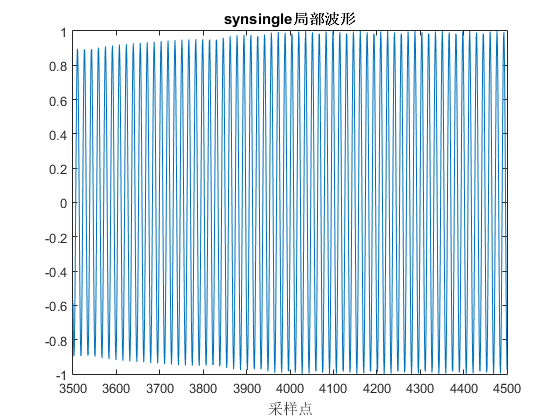
\includegraphics[width=7cm]{figure8.png}
                }
                \caption{synsingle波形}
                \label{fig:synsingle}
            \end{figure}

            时频图:
            \begin{figure}[H]
                \centering
                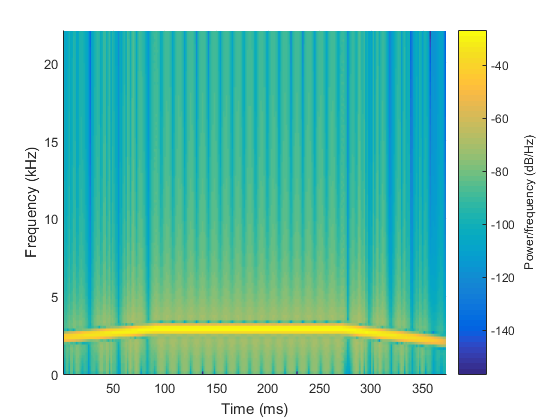
\includegraphics[width=9cm]{figure9.png}
                \label{fig:synsingle-ft}\caption{synsingle时频图}
            \end{figure}

            现在合成的音频在响度、基频变化等方面已经比较接近白鲸的叫声了,但是由于缺少高频分量,声音显得单薄、苍白。

        \subsection{将上述变频信号保存为synsingle.wav文件}

    \section{多变频信号模拟}
        \subsection{认真观察whalesong的时频图,思考什么结构的合成信号能更好的模拟它}
            根据时频图中的功率分布,选取中心频率位于10.875kHz、5.5kHz、8.19kHz的三条谱线,作为高频谐波加入到合成的音频中。

        \subsection{如果允许用多个包络和频率都随时间变化的单频信号模拟白鲸歌声,请描述这些频率变化的特征}
            在上题2.8kHz基频的基础上加入下面的三个谐波分量:
            \subsubsection*{10.875kHz分量}
                12000采样点以后频率由10.875kHz线性减小至8.69kHz。
            \subsubsection*{5.5kHz分量}
                4000采样点以前频率由5.8kHz线性较小至5.5kHz,12000采样点以后频率由5.5kHz线性减小至4.88kHz。
            \subsubsection*{8.19kHz分量}
                4000采样点以前频率由6.25kHz\emph{二次}增加至8.19kHz,12000采样点以后频率有8.19kHz线性减小至5.94kHz。

            对基频和上述3个谐波分量,包络变化与第2题相同。当它们合成为一个音频时,振幅比例为0.8、0.1、0.05、0.05。

        \subsection{用上题结果合成一个多变频信号,绘制波形和时频图,听听声音,解释和白鲸的歌声有何异同}
            合成音频波形如下图所示:
            \begin{figure}[htb]
                \centering
                \subfloat[完整波形]
                {
                    \label{fig:synmulti-1}
                    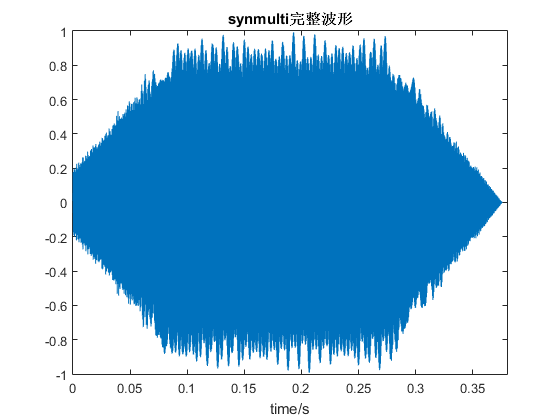
\includegraphics[width=7cm]{figure10.png}
                }
                \hspace{10pt}
                \subfloat[局部波形]
                {
                    \label{fig:synmulti-2}
                    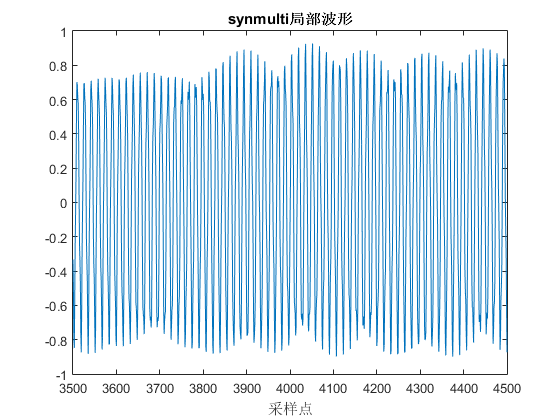
\includegraphics[width=7cm]{figure11.png}
                }
                \caption{synmulti波形}
                \label{fig:synmulti}
            \end{figure}

            时频图:
            \begin{figure}[htb]
                \centering
                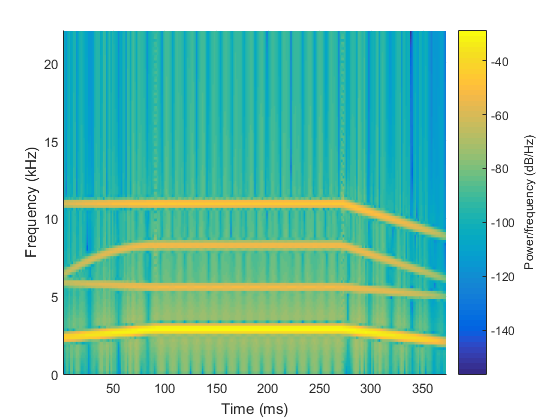
\includegraphics[width=9cm]{figure12.png}
                \label{fig:synmulti-ft}\caption{synmulti时频图}
            \end{figure}

            现在合成的音频已经比较接近白鲸的叫声了。和白鲸的叫声相比,合成的音频听起来非常清晰,而原始音频带有混响,略有模糊感。

        \subsection{将上述单频信号保存为synmulti.wav文件}

    \section{模拟混响效果}
        \subsection{思考如何模拟混响效果}
            海洋馆中的小白鲸处于一个巨大的房间样空间中,混响效果较为明显,在Audition的“卷积混响”设置中,“房间大小”应该较大。另外,白鲸叫声悦耳,因此混响设置中高频衰减较小,低频衰减较大。

        \subsection{使用CoolEdit处理上题的合成音,模拟混响效果,试听结果,并保存为synmultireverb1.wav文件}
            CoolEdit被Adobe公司收购后更名为Audition。这里使用Audition CC 2014对上题合成的音频进行处理。
            
            根据前面的分析,混响参数设置如下:
            \begin{figure}[htb]
                \centering
                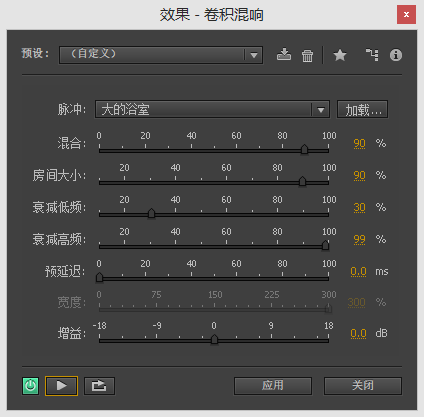
\includegraphics[width=9cm]{figure13.png}
                \label{fig:reverb1-1}\caption{Audition混响设置}
            \end{figure}
            
            处理后的音频波形和时频图如下:
            \begin{figure}[htb]
                \centering
                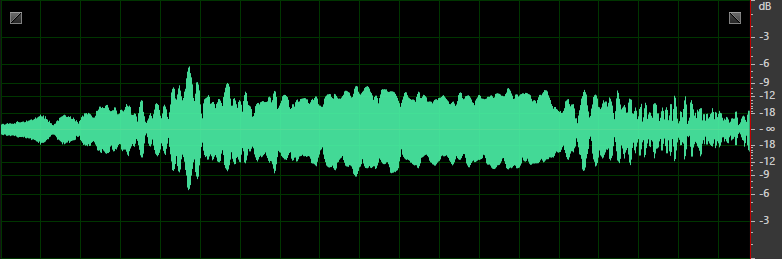
\includegraphics[width=10cm]{figure14.png}
                \label{fig:reverb1-2}\caption{Audition混响波形}
            \end{figure}
            \begin{figure}[htb]
                \centering
                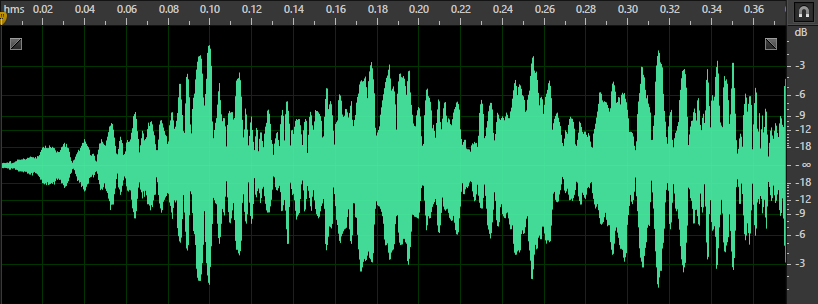
\includegraphics[width=10cm]{figure15.png}
                \label{fig:reverb1-3}\caption{Audition混响时频图}
            \end{figure}
            
        \subsection{设计一个产生混响(产生回声)的滤波器,对上题的合成音进行处理,试听结果,并保存为synmultireverb2.wav文件}
            如下图所示,g(0<g<1)为反馈增益:
            \begin{figure}[htb]
                \centering
                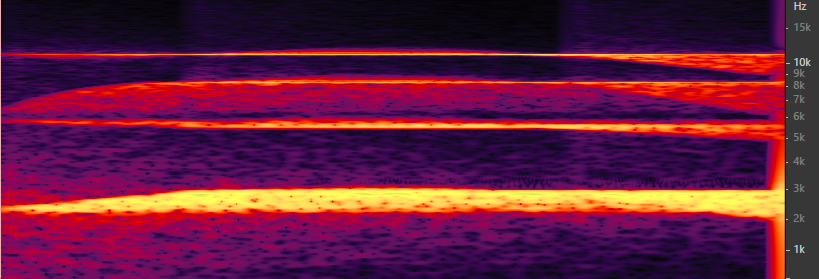
\includegraphics[width=10cm]{figure16.png}
                \label{fig:reverb2-1}\caption{全通滤波器混响模型}
            \end{figure}
            
            该系统的输入输出方程为:
            $$y(n)=-gx(n)+x(n-m)+gy(n-m)$$
            传递函数:
            $$H(z)=\frac{z^{-m}-g}{1-gz^{-m}}$$
            由于$|H(z)|=1$,这是一个全通滤波器混响模型。
            
            取$m=250, g=0.8$,作用于上题合成的音频后,时频图如下图所示:
            \begin{figure}[H]
                \centering
                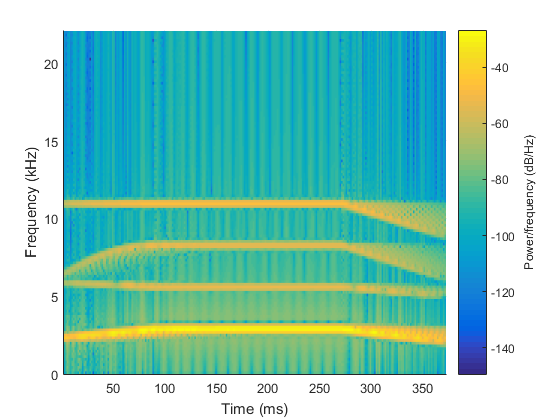
\includegraphics[width=10cm]{figure17.png}
                \label{fig:reverb2-2}\caption{Matlab混响时频图}
            \end{figure}
            
            通过时频图可以确认混响(回声)的存在,但是回声密度不高,混响效果不明显,实际听到音频也是如此。
            
        \subsection{解释混响后的多变频声音和白鲸的歌声有何异同}
            混响后的音频和白鲸的叫声非常相近,但是听起来没有原始音频明亮。这是因为合成音频的过程中,仅选取了能量分布较为集中的3个高频分量,忽略了其他高频分量。高频分量的缺失会使声音听起来略显低沉。
            
\end{document} 